\documentclass[11pt,a4paper]{article}
\usepackage{czt}
\usepackage{graphicx}
\usepackage[parfill]{parskip}
\usepackage{setspace}
\usepackage{hyperref}
\onehalfspacing

\usepackage{lipsum}

\usepackage[utf8]{inputenc}
\usepackage[english]{babel}
\usepackage{csquotes}
\usepackage[backend=biber]{biblatex}
\usepackage{eurosym}
\usepackage{setspace}
\usepackage{enumitem}
\usepackage{afterpage}
\usepackage{float}
\usepackage{caption}
\usepackage{subcaption}
\usepackage{microtype}
\usepackage[T1]{fontenc}
\usepackage[left=3.00cm, right=2.30cm, top=3.00cm, bottom=3.00cm]{geometry}



%\hypersetup{colorlinks, linkcolor=blue, citecolor=blue, linktocpage}
\setstretch{1.25} % 1,25-Facher Zeilenabstand


\title{Verification of Safe and Secure Systems Using Formal Specification}
\author{Andreas Zinkl}

% Top Bar
% % % % % % % % % % % % % % % % % % % % % % % % % % % % % % % % % % % % % % % % % % % % % % % % % % % % 
\usepackage{fancyhdr}
% Clear off all default fancyhdr headers and footers
\fancyhf{}
% Put the page number at the right edge of odd pages, and left edge of even pages.
\fancyhead[RO]{\thepage}
% Custom text at the left edge of odd pages, and right edge of odd pages.
\fancyhead[LO]{\sffamily\itshape Z-Specification}
% Width of the Line
\renewcommand{\headrulewidth}{1pt}
% Apply the fancy header style
\pagestyle{fancy}
% % % % % % % % % % % % % % % % % % % % % % % % % % % % % % % % % % % % % % % % % % % % % % % % % % % % 





\begin{document}
\begin{titlepage}
    \begin{center}
        \vspace*{1cm}
        
        \begin{figure}[H]
			\centering
			\begin{subfigure}{\textwidth}
  				\centering
  				
\includegraphics[width=0.7\linewidth]{images/OTHLogo.jpg}
  				\label{pic:OTHLogo}
			\end{subfigure}%
            \begin{subfigure}{.5\textwidth}
  				\centering
  				
  				\label{pic:HellaLogo}
			\end{subfigure}
		\end{figure}

        
        \vspace{1.7cm}
        
        \Huge
        \textbf{Serving Robot - Formal Z Specification}
        
        \vspace{0.5cm}
        \LARGE
        Verification of Safe and Secure Systems Using Formal Specification
        
        \vspace{3cm}
        
        \textbf{Andreas Zinkl}\\
        \Large
        
        \vspace{1.7cm}
       
        \vfill
        
        Summer Term 2017
        
        \vspace{0.8cm}
          \Large
        Technical Computer Science\\
        Ostbayerische Technische Hochschule Regensburg\\
       \today
        
    \end{center}
\end{titlepage}


\newpage
\fancyhf{} \renewcommand{\headrulewidth}{1pt}
\fancyhead[RO]{\thepage}
\fancyhead[LO]{\sffamily\itshape Contents} 
\tableofcontents
\newpage


% % % % % % % % % % % % % % % % % % % % % % % % % % % % % % % % % % % % % % % % % % % % % % % % % % % % 
% Here starts the specification
% spec-start:
% % % % % % % % % % % % % % % % % % % % % % % % % % % % % % % % % % % % % % % % % % % % % % % % % % % % 

\newpage
\fancyhead[LO]{\sffamily\itshape Introduction}

%SECTION 1 - Introduction
\section{Introduction}
The project "Serving Robot" is about a NXC Lego Mindstorm Robot, which works in a restaurant as a helping robot. The robot helps employees by serving drinks and meals autonomously. The robot is equipped with sensors for route calculation.\\

The restaurant contains the bar and kitchen as well as three tables. The restaurant is split in a grid-layout. The grid-layout defines unique coordinates for every field in the map. The bar, kitchen and the tables are saved in the map as the start position. The map will be used for the navigation of the robot. The navigation algorithm calculates the shortest route to the destination table. The tables are ordered with different priorities. The priority of each table represents the table number. The tables are served in the order of the highest to the lowest priority.\\

The robot can just serve one table at a time. That means, that the robot needs to go back to the bar or kitchen after serving one table. Each table will be marked with one physical and unique coloured line. The robot has a color sensor which recognises the coloured line. If the robot reached the table, he turns around and drives the same way from the table back to the bar or kitchen. The start of the robot needs to be done by a user. This person just needs to press the start button on the robot and the robot starts to work.\\

The restaurant itself is a closed environment. That means, that the robot cannot leave the restaurant. The definition of the restaurant map is done by a text file, which is created by the user. The definition of the map in the text file contains the character '$\#$' as symbols for borders, the character 'S' for the start position and numbers for the table. At the end the map looks like this:

\begin{figure}[!ht]
\centering
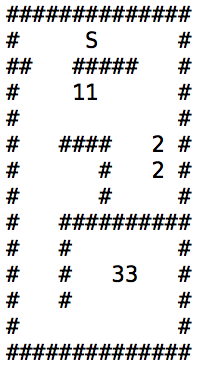
\includegraphics[width=30mm,scale=0.5]{images/map}
\caption{\em The map of the restaurant.}
\label{fig:map}
\end{figure}

%SECTION 2 - Types and Global Variables
\newpage
\fancyhead[LO]{\sffamily\itshape Types and Global Variables}
\section{Types and Global Variables}
The following definitions define important types and global variables which are used over the whole project. The Type DIRECTION represents a command for the robot. Those commands will be sent to the robot and the robot will proceed them. The FreeType FIELD represents all characters which can be set on the map. This can be the position of the robot, the start position of the robot, the position of the borders as well as the positions of each table. Those Types needs to be global, because those are used from the hardware too.

The startposition of the robot is clearly specified and stays the same the whole process. This position also specifies the position of the kitchen / bar which is located as the standard robot startposition. The map of the restaurant is also defined in static values. The room has a static height and width and will not change while the system is running. The specified speed will be sent within a command to the robot. The specified speed limits will always stay the same.

\begin{zed}
[DIRECTION]
\end{zed}
\begin{axdef}
FIELD ::= robotposition | startpoint | tableone | tabletwo | tablethree | border | free | cutlery
\end{axdef}
\begin{axdef}
startposition : (\nat \cross \nat) \pfun FIELD\\
cutlerydesk : (\nat \cross \nat) \pfun FIELD\\
mapWidth : \nat_1\\
mapHeight : \nat_1
\end{axdef}
\begin{axdef}
fullspeed : \power \num\\
halfspeed : \power \num\\
stopspeed : \power \num
\where
\disjoint \langle fullspeed, halfspeed, stopspeed \rangle
\end{axdef}
\begin{axdef}
forward : \power DIRECTION\\
left : \power DIRECTION\\
right : \power DIRECTION\\
turn : \power DIRECTION
\where
\disjoint \langle forward, left, right, turn \rangle
\end{axdef}



%SECTION 3 - System State
\newpage
\fancyhead[LO]{\sffamily\itshape System State Schema}
\section{System State Schema}
\subsection{Defining the System State}
The System State defines the main state of the serving robot. This contains all necessary values like the map and all fields on the \(map\). The map itself is split into various types of fields. Just one type of Fields, called \(free\),  can be used to navigate the robot through the restaurant to the destination table. Tables are a kind of border. A table would be an obstacle which can't be passed without any interaction problems between obstacle and the robot. Borders work like real borders and display walls on the map. The robot needs to circumvent those obastacles. On each serving track, the robot needs to stop at the \(cutlerdesk\). There he picks up the clean cutler which he takes with him to serve the food and drinks. He will also stop at there while driving back from the table to the kitchen, because he will store the used and dirty cutler at the desk for the cleaners.

The track, how the robot needs to drive will be stored as a route. The route is a sequence of coordinates which specify all fields, the robot needs to pass, to get to the destination. The connections between those coordinates are stored in a so called value. The value \(connections\) specify, the link between each field and is necessary to calculate the route to the destination. This also means, that the connection exists not only of \(freefields\). It also contains the \(tables\), which are necessary to identify the destination coordinates of a route.

While the robot is driving, he counts the passed fields in a value called \(drovenFields\). This value is needed to localize the current position, called \(robotpos\), in the map and also to check, which command needs to be executed next. The current position is updated after each driving operation and always up to date.

\begin{schema}{ServingRobotState}

map, robotpos, freefields, borders, tables : (\nat \cross \nat) \pfun FIELD\\
drovenFields : \nat\\
connections : (\nat \cross \nat) \rel (\nat \cross \nat)\\
leftwheelspeed : \num\\
rightwheelspeed : \num

\where

\langle freefields, borders, robotpos} \rangle \partition map \\
\#map = (mapWidth * mapHeight)\\
tables \subset borders\\
\disjoint \langle tables, borders \rangle\\
robotpos \subset freefields\\
\{tableone, tabletwo, tablethree\} \subseteq \ran tables \\
robotpos \in \dom map \\
\#robotpos = 1\\
map(startposition)=startpoint\\
drovenFields <= \#route\\
(\dom freefields \cup \dom talbes) \subseteq \ran connections \\
\dom freefields \subseteq \dom connections
\end{schema}

\newpage
\subsection{Initialization of the System State}
The System State needs an initial state. This state defines the robot without any maps and positions. The robot is standing still in a room. The robot gets its position after starting the system of the robot and defining a map. This needs to be done manually. The robot will be able to start his work, after the system start.

\begin{schema}{InitServingRobotState}
ServingRobotState'
\where
map' = \emptyset \\
connections' = \emptyset\\
freefields' = \emptyset \\
borders' = \emptyset \\
tables' = \emptyset \\
robotpos'  = startposition \\
drovenFields' = 0\\
leftwheelspeed = stopspeed \\
rightwheelspeed = stopspeed
\end{schema}

%SECTION 4 - Operations
\section{Operations}
\fancyhead[LO]{\sffamily\itshape Operations}

The running system for a working restaurant robot needs some important operations and functions. Those define the work logic of the robots and how efficient the robots proceeds his tasks.

%Route Calculation Definition
\subsection{Route Calculation}
The calculation of the route is one of the most important operations, the robot needs to do. The robot can only drive to his destination with a valid route. This valid route is always the best and shortest possible way. It navigates the robot to the tables, where he can serve drinks for the guests. The robot needs to move around the borders and obstacles of the restaurant. The tables on the map can be passed. This is possible because of the small size of the robot, which won't causes interaction problems with the guests. The robot calculates the route, by using the start position and destination coordinates. Those locations are free fields and should be connected by other free fields.\\\\

The \(route!\) will always be the shortest way between the start and the cutlery desk as well as between the cutlery desk and the destination point. For this reason, we can define, that there is no sequence \( betweenRoute \) between the start and the destination which is longer than the current \( betweenRoute \). That means, that we drive through the minimum amount of fields between the given start and destination point. If the given destination is the table, then the calculated destination will be the last \(free\) field in front of the table.\\

Every time, the robot needs to serve a table or comes back from a table to the kitchen, he needs to go the cutlery desk. The cutlery desk is necessary to get the cutlery and plate, which will be used for the meal serving and to store the used cutlery for the cleaners.

\begin{schema}{RouteCalculation}
\Xi ServingRobotState\\
to?, from? : \nat \cross \nat\\
route! : \iseq (\nat \cross \nat)
\where
(from? \in \dom startposition \land to? \in \dom tables)\\
\hspace{20pt}\lor (from? \in \dom tables \land to? \in \dom startposition) \\
(from?, cutlerydesk) \in connections\plus \land (cutlerydesk, to?) \in connections\plus\\\\

\lnot \exists betterRoute : \iseq (\nat \cross \nat) | \\
\hspace{40pt} head~betterRoute = from? \land cutlerydesk \in betterRoute \land last~betterRoute = to?\\
\hspace{10pt} @ \# betterRoute < \# route!\\\\

  \forall i : 1..(\#route!-2)
  \\\hspace{20pt}| route!(i) \in \dom freefields
  \\\hspace{40pt} \land route!(i+1) \in \dom freefields
  \\\hspace{40pt} \land 1 < route!\inv \limg \{cutlerydesk\} \rimg < \# route-1
  \\\hspace{40pt} \land (route!(1) \in startposition \land route!(\#route!) \in \dom tables)
  \\\hspace{20pt}@ (route!(i), route!(i+1)) \in connections
\end{schema}

%Driving Defintion
\subsection{Serve a Table}
If the robot gets the route, he will not know how to drive. The solution for this problem is a sequence of commands. Such commands tell the robot what he needs to do, to reach the destination. The command also calculates the new destination of the robot. The commands are split into driving left, right and forward. The robot does not need to drive backwards. Instead of driving backwards, the robot just turns around 180 degrees and starts driving forward.

\begin{zed}
Drive == DriveLeft \land DriveRight \land DriveForward \land TurnAround\newline
\end{zed}

\subsubsection{Drive Left}
Driving left has 4 special cases. Those ones can be calculated by using the destination field, the actual position and the last droven field. The driving task introduces a state change, which includes the change of the robot position, the speed of the robot as well as the new map. The generated command will be sent to robot with 2 bits, represented by the DIRECTION Type. The current position needs always to be updated. The reason therefore is, because we need to know at which position the robot is standing.

\begin{schema}{DriveLeft}
\Delta ServingRobotState\\
cmd! : DIRECTION\\
route? : \iseq (\nat \cross \nat)
\where
drovenFields < \#route?\\
leftwheelspeed < (rightwheelspeed / 2)\\
\forall m, n : \nat_1 \\
\hspace{20pt} | (m < mapWidth \land n < mapHeight) \land  \\
\hspace{30pt} ( \hspace{5pt} [(m,n+1) = route?(drovenFields-1) \land (m+1,n) = route?(drovenFiels+1)] \lor \\
\hspace{40pt}   [(m-1,n) = route?(drovenFields-1) \land (m,n+1) = route?(drovenFields+1)] \lor \\
\hspace{40pt}   [(m,n-1) = route?(drovenFields-1) \land (m-1,n) = route?(drovenFields+1)] \lor \\
\hspace{40pt}   [(m+1,n) = route?(drovenFields-1) \land (m,n-1) = route?(drovenFields+1)] \hspace{5pt} )\\
\hspace{30pt}@ (m,n) = route?(drovenFields)\\
\\
map' = (map \oplus \{route?(drovenFields) \mapsto freefield,\\ 
\hspace{85pt} route?(drovenFields') \mapsto robotposition\} ) \\\\

drovenFields' = drovenFields+1\\
rightwheelspeed' = fullspeed\\
leftwheelspeed' = halfspeed\\
cmd! = left
\end{schema}

\subsubsection{Drive Right}
Driving right has, as well as driving left, 4 special cases. Those ones can be also calculated by using the destination field, the actual position and the last droven field. The new introduced ServingRobotState includes all changes like in the driving left task. The calculated command will be sent to the robot, to move into the correct position. Driving right is in this way similar to the driving left state.
\begin{schema}{DriveRight}
\Delta ServingRobotState\\
cmd! : DIRECTION\\
route? : \iseq (\nat \cross \nat)
\where
drovenFields < \#route?\\
rightwheelspeed < (leftwheelspeed / 2)\\
\forall m, n : \nat_1 \\
\hspace{20pt} | (m < mapWidth \land n < mapHeight) \land  \\
\hspace{30pt} ( [(m,n+1) = route?(drovenFields-1) \land (m-1,n) = route?(drovenFiels+1)] \lor \\
\hspace{30pt}   [(m-1,n) = route?(drovenFields-1) \land (m,n-1) = route?(drovenFields+1)] \lor \\
\hspace{30pt}   [(m,n-1) = route?(drovenFields-1) \land (m+1,n) = route?(drovenFields+1)] \lor \\
\hspace{30pt}   [(m+1,n) = route?(drovenFields-1) \land (m,n+1) = route?(drovenFields+1)] )\\
\hspace{20pt}@ (m,n) = route?(drovenFields)\\
\\
map' = (map \oplus \{route?(drovenFields) \mapsto freefield,\\ 
\hspace{85pt} route?(drovenFields') \mapsto robotposition\} ) \\\\

drovenFields' = drovenFields+1\\
leftwheelspeed' = fullspeed\\
rightwheelspeed' = halfspeed\\
cmd! = right
\end{schema}

\subsubsection{Drive Forward}
If the robot should drive forward, the robot will always stay on the same row or column on the map. For this calculation, we look also on the last field, the actual position and the destination field. Driving forward introduces like every task a new system state. This is necessary, because the position will change even if the wheelspeed may won't.
\begin{schema}{DriveForward}
\Delta ServingRobotState\\
cmd! : DIRECTION\\
route? : \iseq (\nat \cross \nat)
\where
drovenFields < \#route?\\
leftwheelspeed = rightwheelspeed\\
\forall m, n : \nat_1 \\
\hspace{20pt} | (m < mapWidth \land n < mapHeight) \land  \\
\hspace{20pt} ( [(m,n-1) = route?(drovenFields-1) \land (m,n+1) = route?(drovenFiels+1)] \lor \\
\hspace{30pt}   [(m-1,n) = route?(drovenFields-1) \land (m+1,n) = route?(drovenFields+1)] \lor \\
\hspace{30pt}   [(m,n+1) = route?(drovenFields-1) \land (m,n-1) = route?(drovenFields+1)] \lor \\
\hspace{30pt}   [(m+1,n) = route?(drovenFields-1) \land (m-1,n) = route?(drovenFields+1)] )\\
\hspace{20pt}@ (m,n) = route?(drovenFields)\\
\\
map' = (map \oplus \{route?(drovenFields) \mapsto freefield,\\ 
\hspace{85pt} route?(drovenFields') \mapsto robotposition\} ) \\\\

drovenFields' = drovenFields+1\\
leftwheelspeed'=fullspeed\\
rightwheelspeed'=fullspeed\\
cmd! = forward
\end{schema}


\subsubsection{Destination reached - Turn Around}
After reaching the destination, the robot needs to drive back the whole route. For this, the robot just turns around and uses a new route for the drive back home. This new route will be calculated after the turn. The new route mostly is just just the reverse old route, because this is also the fastest way. The values, which display the robot and route state (meaning the amount of droven fields), will be set to the initial value. The new route will be passed like the old route before, just reverse. Also this tasks introduces a new ServingRobotState. The map stays the same, but the route will be reversed and the wheelspeed, as well as the drovenFields will be changed for this task.
\begin{schema}{TurnAround}
\Delta ServingRobotState\\
cmd! : DIRECTION\\
route? : \iseq (\nat \cross \nat)
\where
drovenFields = \#route?\\
rightwheelspeed = -leftwheelspeed\\
\\
map' = map\\
leftwheelspeed' = -fullspeed\\
rightwheelspeed' = fullspeed\\
drovenFields' = 0\\
cmd! = turn
\end{schema}

\end{document}
